\documentclass[12pt]{article}

\usepackage{amsmath}
\usepackage{amssymb}
\usepackage{xspace}
\usepackage{color}
\usepackage[total={6in,8in}]{geometry}
\usepackage{amsthm}
\usepackage{graphicx}

\usepackage{enumitem}
\usepackage{centernot}
\usepackage[utf8]{inputenc}
\usepackage[english]{babel}
\usepackage{mathrsfs}

\newtheorem{theorem}{Theorem}
\newtheorem{definition}{Definition}
\newcommand{\N}{\mathbb{N}}
\newcommand{\Z}{\mathbb{Z}}
\newcommand{\Q}{\mathbb{Q}}
\newcommand{\R}{\mathbb{R}}
\newcommand{\C}{\mathbb{C}}
\newcommand{\sn}{\mathfrak{S}}
\newcommand{\ve}{\varepsilon}
\newcommand{\ketz}{\ensuremath{\lvert 0\rangle}\xspace}
\newcommand{\keto}{\ensuremath{\lvert 1\rangle}\xspace}
\newcommand{\ket}[1]{\ensuremath{\lvert #1\rangle}\xspace}
\newcommand{\ketpsi}{\ensuremath{|\psi\rangle}\xspace}
\newcommand{\bra}[1]{\ensuremath{\langle #1\vert}\xspace}
\newcommand{\Hplus}{\ensuremath{\lvert + \rangle}\xspace}
\newcommand{\Hminus}{\ensuremath{\lvert- \rangle}\xspace}
\newcommand{\inner}[2]{\ensuremath{\langle #1 \mid #2 \rangle}\xspace}
\newlength{\minuslength}
\settowidth{\minuslength}{$-$}
\newcommand{\hadamard}{
\frac{1}{\sqrt{2}}
\begin{bmatrix}
1 & \hspace{\minuslength}1\\
1 & -1 
\end{bmatrix}
}
\setlength{\parindent}{1cm}


\author{Marika Swanberg}

\begin{document}
\section{Block Sensitivity} 
Block sensitivity is a lower bound on all query complexity measures (?)

\begin{definition}[Block sensitivity] For an input $x\in \{0,1\}^N$ and a subset of variables $S \subseteq \{1, 2, \ldots, N\}$, $x^{(S)}$ is the input obtained from $x$ by changing all $x_i, i \in S$ to opposite values. The block sensitivity $bs(f)$ is the maximum $k$ for which there is an input $x \in \{0,1\}^N$ and pairwise disjoint subsets $S_1, \ldots, S_k \subseteq \{1, \ldots, N\}$ with $f(x) \neq f(x^{(S_i)})$ for all $1 \leq i \leq k$
\end{definition}

What does this mean in the context of error-correcting codes? We want to know the block sensitivity of $f$, our decoding algorithm. For linear decoding, we have $f: \{0,1\}^n \rightarrow \{0,1\}^k$ where the messages are of length $k$ and the codewords have $n-k$ check bits. 

\begin{theorem}
For linear codes $\mathscr{C} = [n,k]$ with minimum distance $d$, the nearest neighbor decoding function $f: \{0,1\}^n \rightarrow \{0,1\}^k$ has a block sensitivity $$
bs(f) \leq \frac{n}{\lfloor \frac{1}{2}(d-1)  \rfloor +1}$$
\end{theorem}

\begin{proof}
Our linear code has minimum distance $d$. By (theorem 2 in MacWilliams and Sloane), the code can correct $\lfloor \frac{1}{2}(d-1) \rfloor$ errors. Thus, $f(x) = f(x^{(S)})$ where $\lvert S \rvert \leq \lfloor \frac{1}{2}(d-1) \rfloor$. Correct decoding is not guaranteed when $\lvert S \rvert > \lfloor \frac{1}{2}(d-1) \rfloor$. There are at most $n/(\lfloor \frac{1}{2}(d-1) \rfloor +1)$ pairwise disjoint sets of size $\lfloor \frac{1}{2}(d-1) \rfloor+ 1$ in $\{1, \ldots, n\}$, which could all potentially lead to decoding errors. Thus, $$bs(f) \leq \frac{n}{\lfloor \frac{1}{2}(d-1)  \rfloor +1}.$$\\
\end{proof}

\section{Certificate Complexity}

For an input $x \in \{0,1\}^N$, a certificate is a set $S \subseteq \{1, \ldots, N\}$ with the property that the variables $x_i, i \in S$ determine the value of $f(x)$. 
 
\begin{definition}[Certificate complexity] $S \subseteq \{1, \ldots, N\}$ is a certificate on an input $x$ if, for any $y \in \{0,1\}^N$ such that $x_i = y_i, i \in S$, we have $f(x) = f(y)$. $C_x(f)$ is the minimum size $\lvert S \rvert$ of a certificate $S$ on input $x$. The certificate complexity $C(f)$ is the maximum of $C_x(f)$ over all $x\in \{0,1\}$.
\end{definition}

\begin{theorem}
For a linear code $\mathscr{C} = [n,k]$ with distance $d$, the nearest neighbor decoding function $f$ has certificate complexity $C(f) = n -d +1$.
\end{theorem}

\begin{proof}
Nearest neighbor decoding relies on the minimum distance $d$ between any two codewords. Our code $\mathscr{C} $ has minimum distance $d$; thus, there exist received codewords $x$ and $y$ with distance $2 \cdot \lfloor \frac{1}{2}(d-1)\rfloor = d-1$ apart (centered around a codeword $u$) in which $f(x) = u = f(y)$. 

Then, the minimum certificate that can exist between $x$ and $y$ is a set $S$ of size $n-(d-1) = n-d+1$. Since $d$ is the minimum distance for $\mathscr{C}$ , we can bound the minimum certificate size for any received codeword $r$ $, C_r(f) \leq n - d +1.$ Thus, the maximum certificate size $C_x(f)$ for all $x \in \{0,1\}^n$, i.e. the total certificate complexity of $\mathscr{C}$ is $n-d+1$.\\
\end{proof}

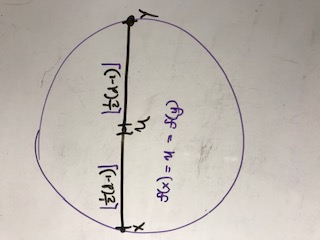
\includegraphics[scale=1, angle=270]{cert_comp_pic.jpg}
\end{document}